\documentclass{standalone}

\usepackage{tikz}
\usepackage{amsmath}
\usetikzlibrary{matrix}
\usetikzlibrary {shapes.geometric}
\usetikzlibrary {positioning}
\usetikzlibrary {decorations.pathmorphing}
\usetikzlibrary {arrows.meta}

\begin{document}
        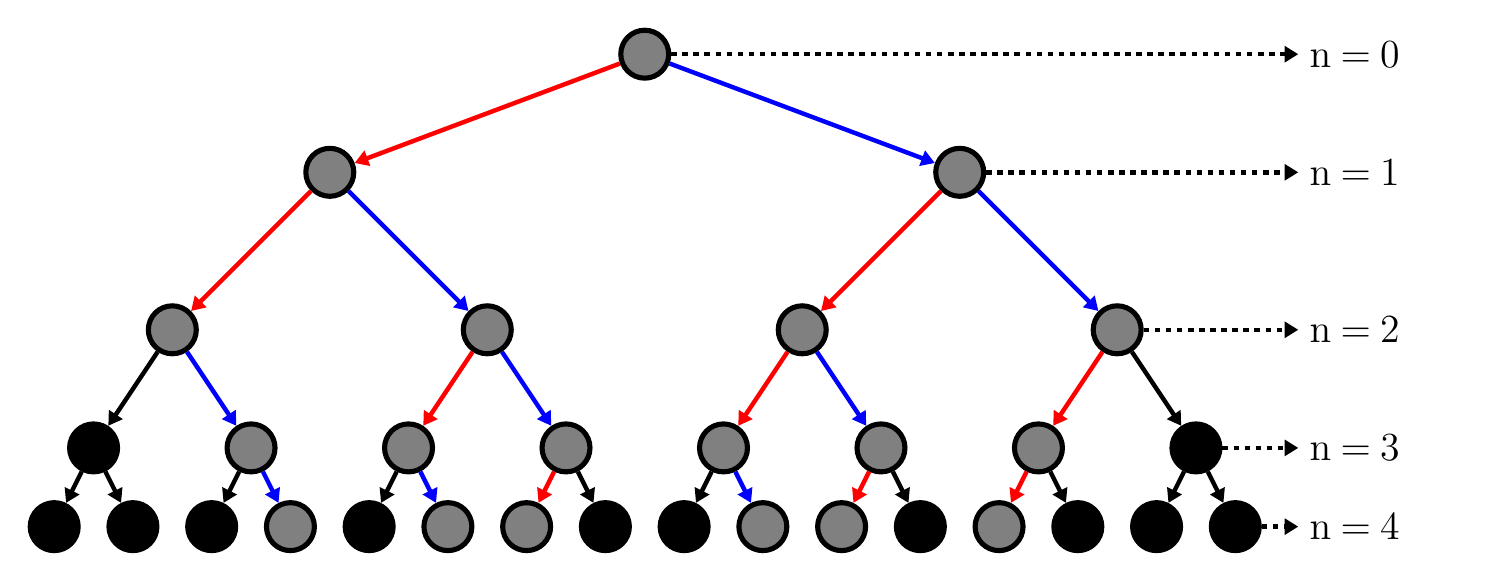
\begin{tikzpicture}[ultra thick]
            

            %\draw [help lines] (0,0) grid (16,5); 

            \path   (7.5,6)  node (a) [circle,draw] {0}
                    (3.5,4.5) node (b) [circle,draw] {0}
                    (11.5,4.5) node (c) [circle,draw] {0}
                    (1.5,2.5) node (d) [circle,draw] {0}
                    (5.5,2.5) node (e) [circle,draw] {0}
                    (9 .5,2.5) node (f) [circle,draw] {0}
                    (13.5,2.5) node (g) [circle,draw] {0}
                    (0.5,1) node (h) [circle,draw] {0}
                    (2.5,1) node (i) [circle,draw] {0}
                    (4.5,1) node (j) [circle,draw] {0}
                    (6.5,1) node (k) [circle,draw] {0}
                    (8.5,1) node (l) [circle,draw] {0}
                    (10.5,1) node (m) [circle,draw] {0}
                    (12.5,1) node (n) [circle,draw] {0}
                    (14.5,1) node (o) [circle,draw] {0}
                    (0,0) node (p) [circle,draw] {0}
                    (1,0) node (q) [circle,draw] {0}
                    (2,0) node (r) [circle,draw] {0}
                    (3,0) node (s) [circle,draw] {0}
                    (4,0) node (t) [circle,draw] {0}
                    (5,0) node (u) [circle,draw] {0}
                    (6,0) node (v) [circle,draw] {0}
                    (7,0) node (w) [circle,draw] {0}
                    (8,0) node (x) [circle,draw] {0}
                    (9,0) node (y) [circle,draw] {0}
                    (10,0) node (z) [circle,draw] {0}
                    (11,0) node (w5) [circle,draw] {0}
                    (12,0) node (w6) [circle,draw] {0}
                    (13,0) node (w7) [circle,draw] {0}
                    (14,0) node (w8) [circle,draw] {0}
                    (15,0) node (w9) [circle,draw] {0};
                    





                    
            \draw [fill=gray] (7.5,6) circle [radius=0.3];
            \draw [fill=gray] (3.5,4.5) circle [radius=0.3];
            \draw [fill=gray] (11.5,4.5) circle [radius=0.3];
            \draw [fill=gray] (1.5,2.5) circle [radius=0.3];
            \draw [fill=gray] (5.5,2.5) circle [radius=0.3];
            \draw [fill=gray] (9 .5,2.5) circle [radius=0.3];
            \draw [fill=gray] (13.5,2.5) circle [radius=0.3];
            \draw [fill=black] (0.5,1) circle [radius=0.3];
            \draw [fill=gray] (2.5,1) circle [radius=0.3];
            \draw [fill=gray] (4.5,1) circle [radius=0.3];
            \draw [fill=gray] (6.5,1) circle [radius=0.3];
            \draw [fill=gray] (8.5,1) circle [radius=0.3];
            \draw [fill=gray] (10.5,1) circle [radius=0.3];
            \draw [fill=gray] (12.5,1) circle [radius=0.3];
            \draw [fill=black] (14.5,1) circle [radius=0.3];
            \draw [fill=black] (0,0) circle [radius=0.3];
            \draw [fill=black] (1,0) circle [radius=0.3];
            \draw [fill=black] (2,0) circle [radius=0.3];
            \draw [fill=gray] (3,0) circle [radius=0.3];
            \draw [fill=black] (4,0) circle [radius=0.3];
            \draw [fill=gray] (5,0) circle [radius=0.3];
            \draw [fill=gray] (6,0) circle [radius=0.3];
            \draw [fill=black] (7,0) circle [radius=0.3];
            \draw [fill=black] (8,0) circle [radius=0.3];
            \draw [fill=gray] (9,0) circle [radius=0.3];
            \draw [fill=gray] (10,0) circle [radius=0.3];
            \draw [fill=black] (11,0) circle [radius=0.3];
            \draw [fill=gray] (12,0) circle [radius=0.3];
            \draw [fill=black] (13,0) circle [radius=0.3];
            \draw [fill=black] (14,0) circle [radius=0.3];
            \draw [fill=black] (15,0) circle [radius=0.3];
           
            


            \draw[arrows = -{Triangle[open,angle=60:2mm,fill = red]},red] (node cs: name =a ) -- (node cs:name =b);
            \draw[arrows = -{Triangle[open,angle=60:2mm,fill = blue]},blue] (node cs: name =a ) -- (node cs:name =c);
            \draw[arrows = -{Triangle[open,angle=60:2mm,fill = red]},red] (node cs: name =b ) -- (node cs:name =d);
            \draw[arrows = -{Triangle[open,angle=60:2mm,fill = blue]},blue] (node cs: name =b ) -- (node cs:name =e);
            \draw[arrows = -{Triangle[open,angle=60:2mm,fill = red]},red] (node cs: name =c ) -- (node cs:name =f);
            \draw[arrows = -{Triangle[open,angle=60:2mm,fill = blue]},blue] (node cs: name =c ) -- (node cs:name =g);
            \draw[arrows = -{Triangle[open,angle=60:2mm,fill = black]},black] (node cs: name =d ) -- (node cs:name =h);
            \draw[arrows = -{Triangle[open,angle=60:2mm,fill = red]},red] (node cs: name =e ) -- (node cs:name =j);
            \draw[arrows = -{Triangle[open,angle=60:2mm,fill = red]},red] (node cs: name =f ) -- (node cs:name =l);
            \draw[arrows = -{Triangle[open,angle=60:2mm,fill = red]},red] (node cs: name =g) -- (node cs:name =n);
            \draw[arrows = -{Triangle[open,angle=60:2mm,fill = blue]},blue] (node cs: name =d ) -- (node cs:name =i);
            \draw[arrows = -{Triangle[open,angle=60:2mm,fill = blue]},blue] (node cs: name =e ) -- (node cs:name =k);
            \draw[arrows = -{Triangle[open,angle=60:2mm,fill = blue]},blue] (node cs: name =f) -- (node cs:name =m);
            \draw[arrows = -{Triangle[open,angle=60:2mm,fill = black]},black] (node cs: name =g ) -- (node cs:name =o);
            \draw[arrows = -{Triangle[open,angle=60:2mm,fill = black]},black] (node cs: name =h ) -- (node cs:name =p);
            \draw[arrows = -{Triangle[open,angle=60:2mm,fill = black]},black] (node cs: name =h ) -- (node cs:name =q);
            \draw[arrows = -{Triangle[open,angle=60:2mm,fill = black]},black] (node cs: name =i ) -- (node cs:name =r);
            \draw[arrows = -{Triangle[open,angle=60:2mm,fill = blue]},blue] (node cs: name =i ) -- (node cs:name =s);
            \draw[arrows = -{Triangle[open,angle=60:2mm,fill = black]},black] (node cs: name =j ) -- (node cs:name =t);
            \draw[arrows = -{Triangle[open,angle=60:2mm,fill = blue]},blue] (node cs: name =j ) -- (node cs:name =u);
            \draw[arrows = -{Triangle[open,angle=60:2mm,fill = red]},red] (node cs: name =k ) -- (node cs:name =v);
            \draw[arrows = -{Triangle[open,angle=60:2mm,fill = black]},black] (node cs: name =k ) -- (node cs:name =w);
            \draw[arrows = -{Triangle[open,angle=60:2mm,fill = black]},black] (node cs: name =l ) -- (node cs:name =x);
            \draw[arrows = -{Triangle[open,angle=60:2mm,fill = blue]},blue] (node cs: name =l ) -- (node cs:name =y);
            \draw[arrows = -{Triangle[open,angle=60:2mm,fill = red]},red] (node cs: name =m ) -- (node cs:name =z);
            \draw[arrows = -{Triangle[open,angle=60:2mm,fill = black]},black] (node cs: name =m ) -- (node cs:name = w5);
            \draw[arrows = -{Triangle[open,angle=60:2mm,fill = red]},red] (node cs: name =n ) -- (node cs:name = w6);
            \draw[arrows = -{Triangle[open,angle=60:2mm,fill = black]},black] (node cs: name =n ) -- (node cs:name = w7);
            \draw[arrows = -{Triangle[open,angle=60:2mm,fill = black]},black] (node cs: name =o ) -- (node cs:name =w8);
            \draw[arrows = -{Triangle[open,angle=60:2mm,fill = black]},black] (node cs: name =o ) -- (node cs:name =w9);

            \draw[arrows = -{Triangle[open, angle=60:2mm,fill=black]}] [dash pattern=on 2pt off 2pt](node cs: name =a ) -- (15.8,6);
            \draw[arrows = -{Triangle[open, angle=60:2mm,fill=black]}] [dash pattern=on 2pt off 2pt](node cs: name =c ) -- (15.8,4.5);
            \draw[arrows = -{Triangle[open, angle=60:2mm,fill=black]}] [dash pattern=on 2pt off 2pt](node cs: name =g ) -- (15.8,2.5);
            \draw[arrows = -{Triangle[open, angle=60:2mm,fill=black]}] [dash pattern=on 2pt off 2pt](node cs: name =o ) -- (15.8,1);
            \draw[arrows = -{Triangle[open, angle=60:2mm,fill=black]}] [dash pattern=on 2pt off 2pt](node cs: name =w9 ) -- (15.8,0);

            \node [right=8.3cm,text width=2cm] at (a)
            {
            \mbox{\Large n = 0}
            };

            \node [right=4.3cm,text width=2cm] at (c)
            {
            \mbox{\Large n = 1}
            };

            \node [right=2.3cm,text width=2cm] at (g)
            {
            \mbox{\Large n = 2}
            };

            \node [right=1.3cm,text width=2cm] at (o)
            {
            \mbox{\Large n = 3}
            };

            \node [right=0.8cm,text width=2cm] at (w9)
            {
            \mbox{\Large n = 4}
            };
        \end{tikzpicture}
\end{document}